\subsubsection{الگوی \lr{Hierarchical Control}}
\label{archHierContSec}
\begin{RTL}
الگوی کنترل سلسله‌مراتبی \cite{ref4} یک
نسخه تخصصی از \nameref{archRecContainSec}
است که الگوریتم‌های پیچیده کنترلی را بین اجزای مختلف توزیع می‌کند.
این الگو از دو نوع واسط استفاده می‌کند:
واسط‌های کنترلی که نحوه دستیابی به رفتارها را نظارت و کنترل می‌کنند
و واسط‌های عملکردی که خدمات کنترل‌شده توسط واسط‌های دیگر را فراهم می‌کنند.
واسط‌های کنترلی کیفیت خدمات، مانند دقت و صحت، را تعیین می‌کنند
و سیاست‌های اجرایی را تنظیم می‌کنند. واسط‌های عملکردی رفتار مطلوب
را با استفاده از کیفیت خدمات و سیاست‌های تنظیم شده توسط واسط
کنترلی اجرا می‌کنند. این الگو با استفاده از نمودارهای حالت برای
هماهنگی اجزای زیرمجموعه و تجمیع اجزای جزء به کنترل‌کننده
از طریق ترکیب، ساختار سلسله‌مراتبی قابل تنظیم و مقیاس‌پذیری را
فراهم می‌کند. در این الگو، کنترل‌کننده وظیفه هماهنگی درخواست‌های
خدمات به عناصر جزء را دارد و اغلب از نمودارهای حالت برای نشان
دادن حالت‌های تنظیمات اجزای زیرمجموعه استفاده می‌کند. این روش
به ویژه زمانی مفید است که حالت‌های مختلف اجزای زیرمجموعه مستقل
نباشند و با استفاده از نمودارهای حالت و انطباق حالت‌ها، سازگاری میان اجزا حفظ شود.
\end{RTL}
\begin{figure}[h!]
\centering
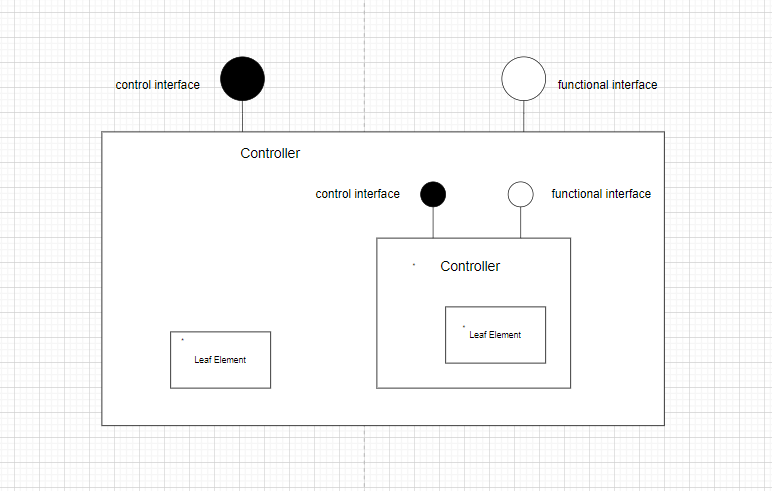
\includegraphics[scale=0.5]{images/first/hierarchical.png}
\caption{ساختار الگوی \lr{Hierarchical Control}}
\end{figure}